\RequirePackage[l2tabu, orthodox]{nag}
\documentclass{article}

\newcounter{chapter}
\setcounter{chapter}{1}
\setcounter{section}{0}

\usepackage{amssymb,amsmath,verbatim,graphicx,microtype,units,booktabs}
\usepackage[margin=10pt, font=small, labelfont=bf, labelsep=endash]{caption}
\usepackage[colorlinks=true, pdfborder={0 0 0}]{hyperref}
\usepackage[utf8]{inputenc}
\usepackage{pdfpages}

\usepackage[left=0.75in, right=0.75in]{geometry}
\usepackage{titleps}
\newpagestyle{main}{
    \setheadrule{.4pt}
    \sethead{Chapter \thechapter: \sectiontitle}
            {}
            {Illya Starikov}
}
\pagestyle{main}

\begin{document}
\section{The Study of the Mind}
\subsection{Study Guide Material}
\begin{itemize}
    \item In 1879, \textbf{William Wundt} started the first formal psychology lab in Leipzig.
    \item \textbf{Structuralism} is where we analyze consciousness.
    \item \textbf{Introspection} is self observation, self awareness.
    \item \textbf{Functionalism} worried about the purpose of consiouness, the why.
    \item \textbf{Sigmund Freud} was big on the unconscious. **Unconscious** is thoughts, memories, desires. He thought that our unconscious governed our behavior. Our thoughts memories, desires, thoughts make us do what we do. He introduced **Psychoanalytic theory** focuses on studying the unconscious --- interpreting dreams as an example. ``People are not masters of their own minds''. Proposed behavior is people coping with sexual urges.
    \item \textbf{Behaviorism} described by Watson.
    \item \textbf{BF Skinner} Famous for saying ``Free will is an illusion''. We have no free will, controlled by our environment.
    \item \textbf{Humanism} Unique aspects of human experience. Humans are free, rational beings with the potential for personal growth, and they are fundamentally different from animals.
    \item \textbf{Applied and clinical psychology}
    \begin{itemize}
        \item \textit{Applied} is like the talk therapy. Psychologist.
        \item \textit{Clinical} is the   and treating the symptoms. Psychiatrist, going to the doctor.
    \end{itemize}
    \item \textbf{Cognition} Refers to mental process to acquire knowledge.
    \item \textbf{Areas of psychology}
\end{itemize}

\begin{center}
    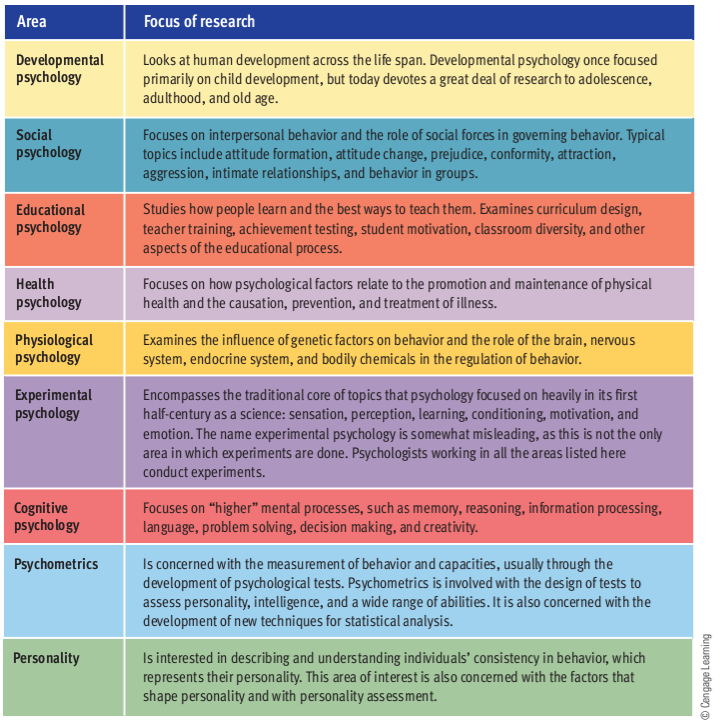
\includegraphics{areas.png}
\end{center}

\begin{itemize}
    \item \textbf{7 unifying themes}
    \begin{enumerate}
        \item Psychology is empirical --- we learn through observation.
        \item Psychology is the theoretical diverse --- different collections of observations
        \item Psychology evolves in a socio-historical context --- different trends have evolved.
        \item Behavior is determined by multiple causes ---
        \item Behavior is shaped by cultural heritage.
        \item Heredity and environment jointly influence behavior.
        \item People's experience of the world is highly subjective.
    \end{enumerate}

    \item \textbf{John B. Watson} was a behaviorist. We should study observable behavior. People watching. Didn't like freud --- wanted to ban all unconscious studying. Big nature vs. nurture.
\end{itemize}

\subsection{Book Notes}
\begin{center}
    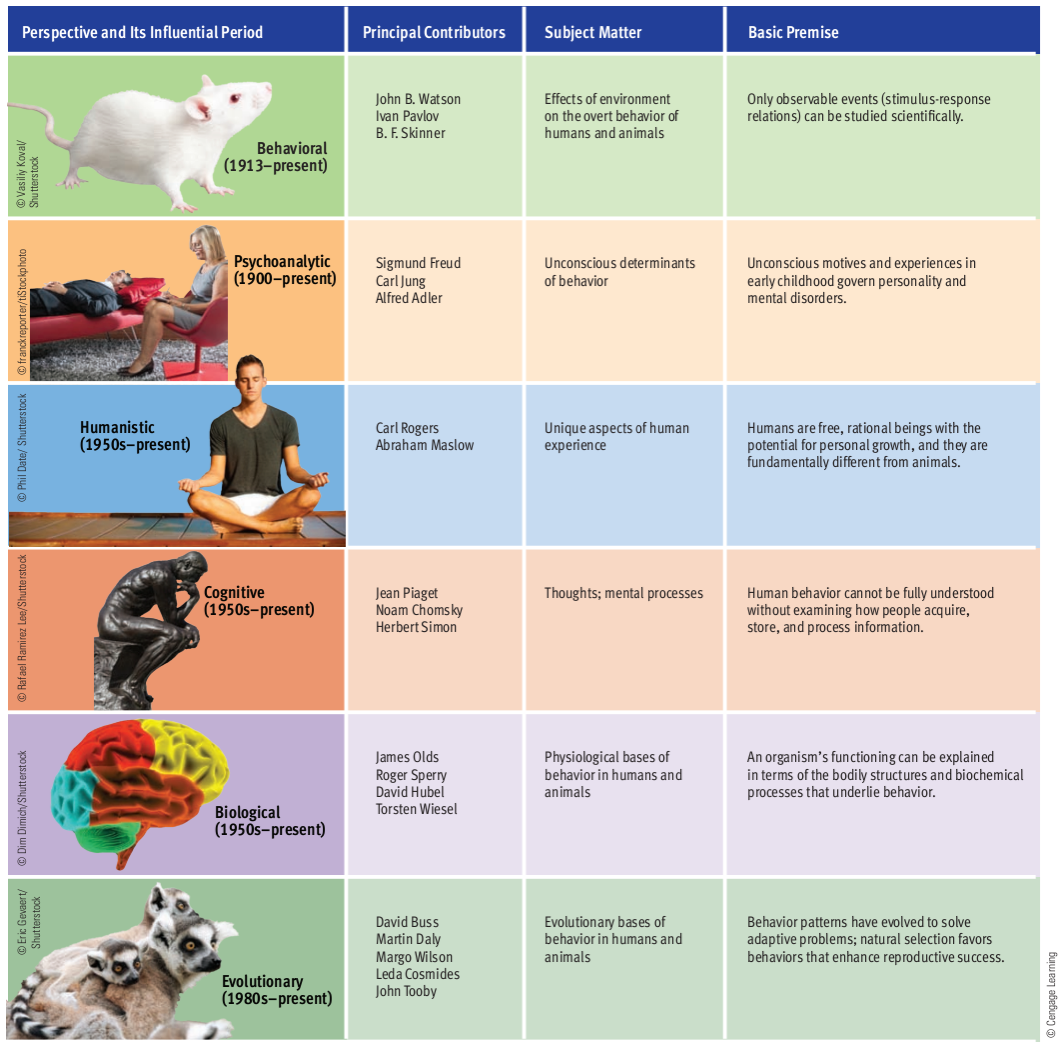
\includegraphics[width=\textwidth]{types.png}
\end{center}

\subsection{Powerpoint Notes}
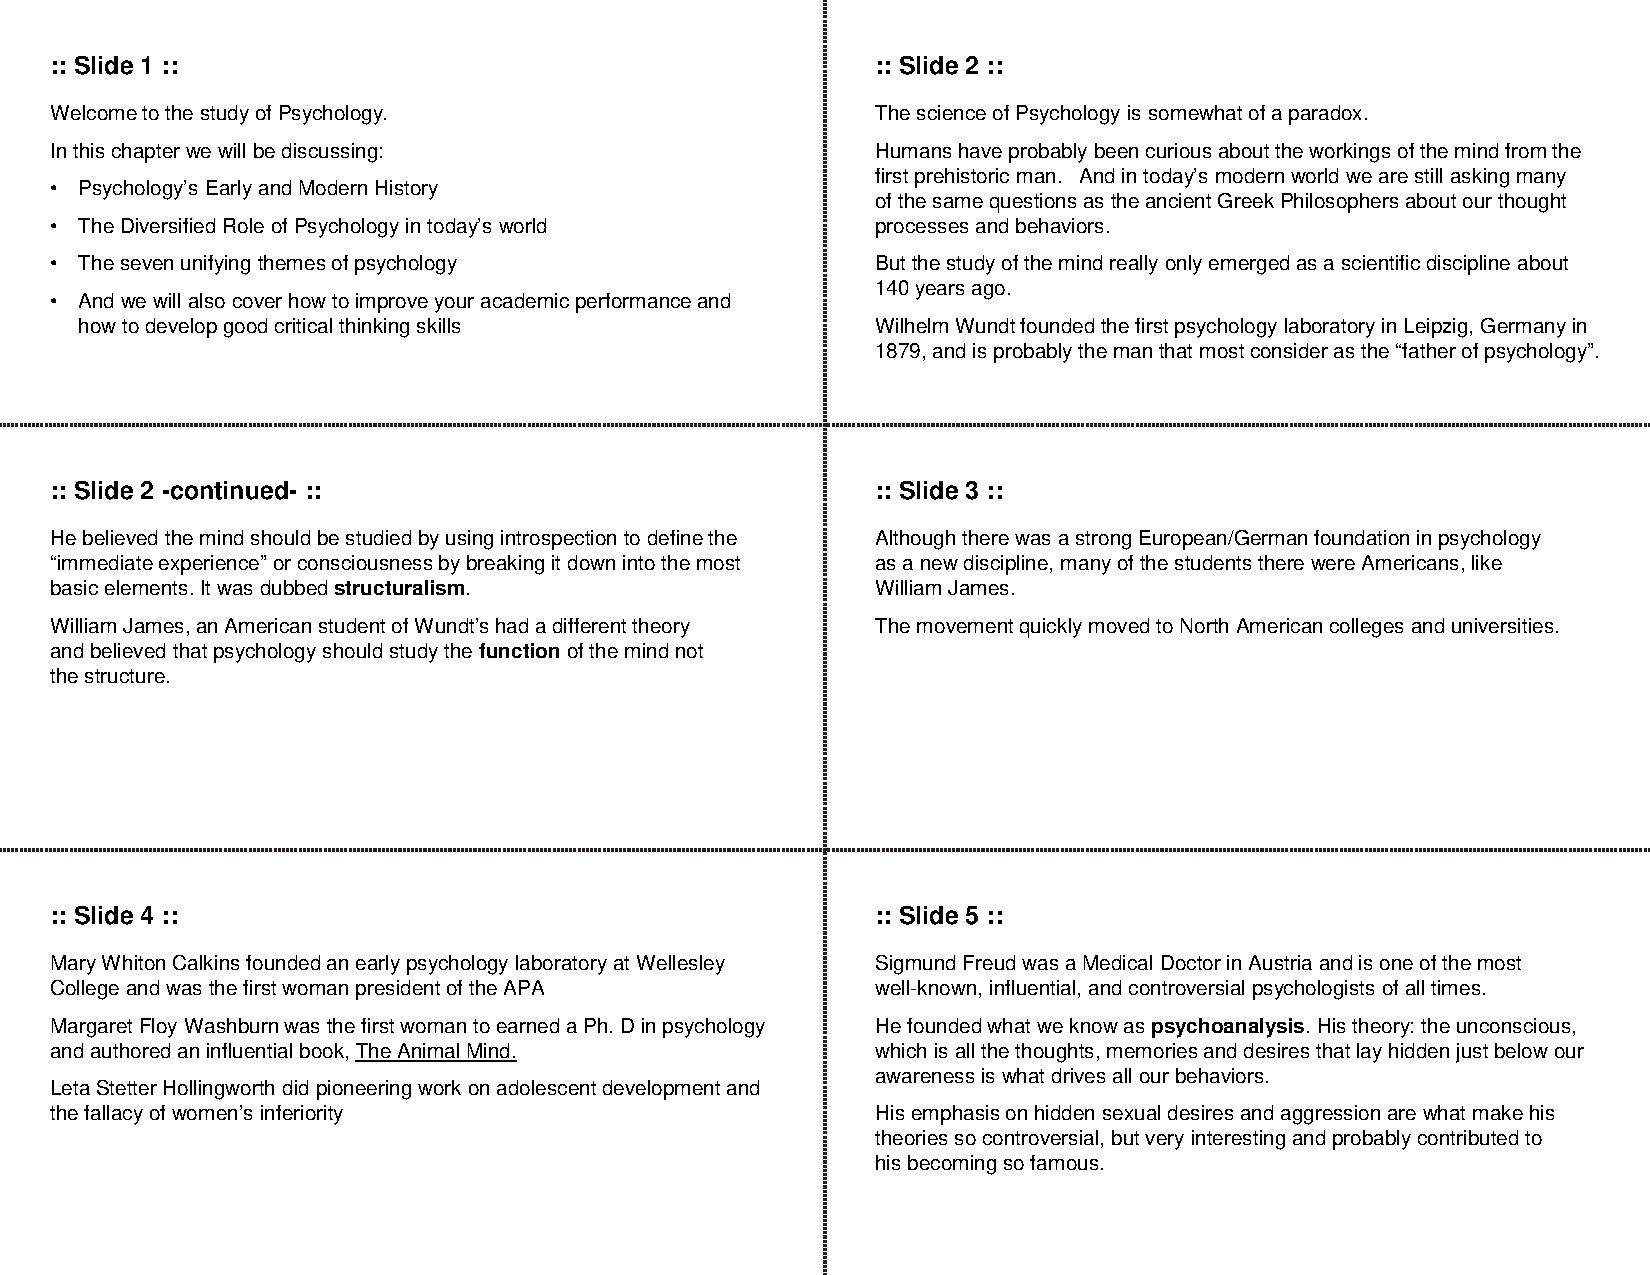
\includepdf[width=1.15\textwidth, pages=-]{lecture_notes_1.pdf}

\end{document}